\documentclass[11pt,a4paper]{article}

% ==============================================================================
% PACKAGES & CONFIGURATION
% ==============================================================================
\usepackage[utf8]{inputenc}
\usepackage[margin=1in]{geometry}
\usepackage{amsmath,amssymb,amsfonts}
\usepackage{graphicx}
\usepackage{booktabs}
\usepackage{tabularx}
\usepackage{longtable}
\usepackage{array}
\usepackage{xcolor}
\usepackage{hyperref}
\usepackage{fancyhdr}
\usepackage{titlesec}
\usepackage{listings}
\usepackage{caption}
\usepackage{subcaption}
\usepackage{float}
\usepackage{tikz}
\usepackage{pgfgantt}
\usetikzlibrary{shapes.geometric, arrows.meta, positioning, calc, fit, backgrounds, shadows}

% Hyperlink configuration
\hypersetup{
    colorlinks=true,
    linkcolor=blue!80!black,
    citecolor=green!60!black,
    urlcolor=blue!70!black,
    pdftitle={Final Capstone Project Proposal - MediPulse AI},
    pdfauthor={Khalid Mansoor}
}

% Color Definitions
\definecolor{primaryblue}{RGB}{30, 58, 138}
\definecolor{secondaryteal}{RGB}{15, 118, 110}
\definecolor{darkgray}{RGB}{51, 65, 85}
\definecolor{lightgray}{RGB}{241, 245, 249}
\definecolor{codebg}{RGB}{248, 250, 252}

% Code Listing Settings
\lstset{
    backgroundcolor=\color{codebg},
    basicstyle=\ttfamily\footnotesize,
    keywordstyle=\color{blue}\bfseries,
    stringstyle=\color{teal},
    commentstyle=\color{gray}\itshape,
    numbers=left,
    numberstyle=\tiny\color{gray},
    stepnumber=1,
    numbersep=8pt,
    frame=single,
    rulecolor=\color{lightgray},
    breaklines=true,
    showstringspaces=false,
    tabsize=2,
    captionpos=b
}

% Header and Footer
\pagestyle{fancy}
\fancyhf{}
\rhead{\footnotesize \textcolor{darkgray}{Final Capstone Proposal -- MediPulse AI}}
\lhead{\footnotesize \textcolor{darkgray}{Department of Computer Science \& Engineering}}
\rfoot{\footnotesize Page \thepage}
\lfoot{\footnotesize \textcolor{darkgray}{Part I: Proposal \& Prototyping}}
\renewcommand{\headrulewidth}{0.4pt}
\renewcommand{\footrulewidth}{0.4pt}

% Section Title Styling
\titleformat{\section}{\large\bfseries\color{primaryblue}}{\thesection}{1em}{}[\titlerule]
\titleformat{\subsection}{\normalsize\bfseries\color{secondaryteal}}{\thesubsection}{1em}{}
\titleformat{\subsubsection}{\small\bfseries\color{darkgray}}{\thesubsubsection}{1em}{}

% TikZ Styles for UML & Software Engineering Diagrams
\tikzset{
    % General
    font=\sffamily\small,
    >=Stealth,
    % DFD Styles
    dfdProcess/.style={circle, draw=primaryblue, thick, fill=blue!5, align=center, minimum size=1.8cm, inner sep=2pt},
    dfdEntity/.style={rectangle, draw=darkgray, thick, fill=gray!10, align=center, minimum width=2.2cm, minimum height=1.1cm},
    dfdStore/.style={rectangle, draw=secondaryteal, thick, fill=teal!5, align=center, minimum width=2.5cm, minimum height=0.9cm},
    % Use Case Styles
    actor/.style={circle, draw=black, thick, fill=white, minimum size=0.6cm, inner sep=0pt},
    usecase/.style={ellipse, draw=primaryblue, thick, fill=blue!5, align=center, minimum width=3.2cm, minimum height=1.1cm},
    systembox/.style={rectangle, draw=darkgray, thick, dashed, inner sep=12pt},
    % Activity Diagram Styles
    activityStart/.style={circle, draw=black, fill=black, minimum size=0.5cm},
    activityEnd/.style={circle, draw=black, double, double distance=1pt, fill=black, minimum size=0.55cm},
    activityAction/.style={rectangle, rounded corners=6pt, draw=primaryblue, thick, fill=blue!5, align=center, minimum width=2.5cm, minimum height=0.9cm},
    activityDecision/.style={diamond, draw=orange!80!black, thick, fill=orange!10, aspect=1.8, align=center, inner sep=2pt},
    % Class Diagram Styles
    umlClass/.style={rectangle, draw=primaryblue, thick, fill=white, align=left, inner sep=6pt},
    % Object Diagram Styles
    umlObject/.style={rectangle, draw=secondaryteal, thick, fill=teal!5, align=left, inner sep=6pt}
}

% ==============================================================================
% DOCUMENT BEGINS
% ==============================================================================
\begin{document}

% ------------------------------------------------------------------------------
% TITLE PAGE
% ------------------------------------------------------------------------------
\begin{titlepage}
    \centering
    \vspace*{1cm}
    
    {\Huge \bfseries \color{primaryblue} MediPulse AI\par}
    \vspace{0.4cm}
    {\Large \bfseries Intelligent Clinical Workflow Automation, Telehealth Triage, \\ and Electronic Health Records Ecosystem\par}
    \vspace{0.8cm}
    {\large \textbf{Final Capstone Project Proposal and Prototyping (Part I)}\par}
    
    \vspace{1.5cm}
    \rule{\linewidth}{1.2pt}
    \vspace{0.5cm}
    
    \begin{minipage}{0.5\textwidth}
        \begin{flushleft} \large
            \textbf{Submitted By:}\\
            \textbf{Student Name:} Khalid Mansoor\\
            \textbf{Student ID:} 2021-CS-88910\\
            \textbf{Program:} B.Sc. in Computer Science \& Engineering\\
            \textbf{Email:} khalid.mansoor@university.edu
        \end{flushleft}
    \end{minipage}
    \begin{minipage}{0.48\textwidth}
        \begin{flushright} \large
            \textbf{Course Code:} CSE-499\\
            \textbf{Course Title:} Final Capstone Project\\
            \textbf{Submission Due:} Wednesday by 11:59 PM\\
            \textbf{Evaluation Points:} 30 Points\\
            \textbf{Deliverable:} GitHub Repository \& Proposal
        \end{flushright}
    \end{minipage}
    
    \vspace{1.5cm}
    \rule{\linewidth}{1.2pt}
    
    \vfill
    
    \textbf{Department of Computer Science and Engineering}\\
    Faculty of Electrical and Computer Engineering\\
    Academic Year 2026--2027\\[0.5cm]
    \today
\end{titlepage}

\newpage
\tableofcontents
\newpage
\listoffigures
\listoftables
\newpage

% ==============================================================================
% EXECUTIVE SUMMARY / ABSTRACT
% ==============================================================================
\section*{Executive Summary}
\addcontentsline{toc}{section}{Executive Summary}
Modern healthcare infrastructure faces an acute dual crisis: clinical workflow congestion and diagnostic triage latency. In emergency and outpatient departments, delayed patient assessment often leads to preventable clinical deterioration, whereas healthcare providers spend up to 45\% of their daily routine on administrative charting and prescription reconciliation. 

\textbf{MediPulse AI} is an intelligent, scalable, and decentralized clinical automation platform designed to bridge the gap between patient self-reporting, automated urgency triaging, real-time physician tele-consultation, and synchronized Electronic Health Record (EHR) management. Built upon robust Object-Oriented Software Engineering principles and governed by an Agile Scrum methodology, this capstone project delivers:
\begin{enumerate}
    \item A machine-assisted clinical decision support triage engine that categorizes patient urgency levels (\textit{Critical}, \textit{Urgent}, \textit{Routine}) and routes patients to appropriate specialist physicians.
    \item A comprehensive Unified Modeling Language (UML) structural and behavioral specification comprising Data Flow Diagrams (Level 0 and 1), Use Case Diagrams, Activity Diagrams, Entity-Relationship Diagrams (ERD), Class Diagrams, and Object Diagrams.
    \item A complete, working, object-oriented prototype implementing at least six core domain classes (\texttt{User}, \texttt{Patient}, \texttt{Doctor}, \texttt{Appointment}, \texttt{MedicalRecord}, \texttt{Prescription}, and \texttt{TriageEngine}) with interactive web and console execution interfaces.
    \item An empirical project completion timeline featuring a Work Breakdown Structure (WBS), sprint milestones, deliverables matrix, and a production Gantt chart.
\end{enumerate}
This proposal details the software engineering specifications, architectural modeling, feasibility analyses, and prototype validation required for Part I of the Senior Capstone Project.

% ==============================================================================
% CHAPTER 1: INTRODUCTION & PROJECT OVERVIEW
% ==============================================================================
\section{Introduction \& Project Overview}

\subsection{Background and Motivation}
The global healthcare ecosystem is experiencing unprecedented operational strain. Escalating chronic disease prevalence, coupled with physician shortages, has led to prolonged outpatient waiting times and clinical burnout. Traditional Hospital Information Systems (HIS) and Electronic Health Record (EHR) platforms are often monolithic, rigid, and disconnected from the patient's immediate triage journey. Patients frequently experience confusion regarding which medical specialty to consult, leading to inappropriate emergency room visits or dangerous delays in acute intervention.

Recent developments in algorithmic clinical decision support and tele-health protocols present an opportunity to automate and optimize these front-door clinical pathways. By embedding algorithmic severity scoring within patient-facing digital portals, healthcare facilities can automate appointment allocation, streamline physician encounter workflows, and ensure cryptographically verifiable digital prescriptions.

\subsection{Problem Statement}
Existing clinical management software architectures suffer from three critical bottlenecks:
\begin{enumerate}
    \item \textbf{Subjective and Delayed Triage:} Patient symptom self-reporting lacks systematic urgency stratification prior to physical or tele-health check-in, resulting in suboptimal resource allocation.
    \item \textbf{Data Fragmentation in Outpatient Encounters:} Diagnostic findings, dynamic physiological vitals, and therapeutic prescriptions are frequently segregated across disjoint databases, requiring manual duplicate data entry by physicians.
    \item \textbf{Lack of Modern, Modular Object-Oriented Extensibility:} Legacy platforms struggle to integrate modern AI-assisted diagnostic assistants and mobile micro-services due to tightly-coupled procedural architectures.
\end{enumerate}

\subsection{Proposed Solution: MediPulse AI}
\textbf{MediPulse AI} addresses these challenges through a modular, object-oriented, patient-centric ecosystem. The system features:
\begin{itemize}
    \item An automated \textbf{Triage Evaluation Engine} assessing symptom acuity and vital signs.
    \item Dynamic \textbf{Physician Matching and Appointment Dispatch} prioritizing acute patients.
    \item An integrated \textbf{Clinical Encounter Workspace} enabling physicians to review vitals, document diagnoses, and digitally sign structured prescriptions in a unified flow.
    \item A cohesive \textbf{Electronic Health Record (EHR) Repository} persisting immutable clinical histories.
\end{itemize}

\subsection{Project Scope and System Boundaries}
\subsubsection{In-Scope Capabilities (Phase I \& II)}
\begin{itemize}
    \item Multi-role role-based access control (Patients, Physicians, Clinical Administrators).
    \item Algorithmic symptom evaluation and triage classification into standardized severity tiers.
    \item Interactive appointment scheduling with conflict prevention and specialty filtering.
    \item Structured digital prescription generation including drug dosages, frequencies, and administration instructions.
    \item Full UML structural and behavioral specifications and operational object-oriented prototype.
\end{itemize}

\subsubsection{Out-of-Scope Capabilities (Delimited for Future Extensions)}
\begin{itemize}
    \item Autonomous robotic surgical control or direct automated drug dispensing hardware.
    \item Native biometric laboratory hardware drivers (simulated via standardized REST/JSON APIs).
    \item Full nationwide health insurance clearinghouse transaction billing settlement.
\end{itemize}

% ==============================================================================
% CHAPTER 2: LITERATURE REVIEW & FEASIBILITY ANALYSIS
% ==============================================================================
\section{Literature Review \& Feasibility Analysis}

\subsection{Comparative Analysis of Existing Systems}
To establish the competitive advantage of MediPulse AI, existing industry platforms were analyzed, as summarized in Table~\ref{tab:comp_analysis}.

\begin{table}[H]
\centering
\caption{Comparative Analysis: MediPulse AI vs. Existing Healthcare Platforms}
\label{tab:comp_analysis}
\small
\begin{tabularx}{\textwidth}{lXXXX}
\toprule
\textbf{Feature} & \textbf{Epic Systems} & \textbf{Cerner (Oracle)} & \textbf{Teladoc Health} & \textbf{MediPulse AI (Proposed)} \\
\midrule
Target Domain & Tier-1 Enterprise & Enterprise Hospital & Virtual Consultations & Integrated Triage \& EHR \\
Triage Automation & Rule-based static & Manual nursing input & Questionnaire-based & Algorithmic Multi-factor AI \\
Architecture & Monolithic / Legacy & Hybrid Cloud & Microservices & Modular OOP Microservices \\
EHR Integration & Comprehensive & Comprehensive & Limited/Third-party & Fully Integrated Encounters \\
Prescription Flow & Complex E-Prescribe & Proprietary CPOE & Basic PDF generation & Verified Digital Prescription \\
Open Prototyping & Closed Source & Closed Source & Closed Source & Open-Standard Academic Prototype \\
\bottomrule
\end{tabularx}
\end{table}

\subsection{Multi-Dimensional Feasibility Study}

\subsubsection{Technical Feasibility}
The system leverages modern, high-performance, and standardized technologies. The domain logic is structured using Python 3.11 and ECMAScript 6+ Object-Oriented classes, ensuring platform independence. Modern relational database management systems (PostgreSQL) coupled with RESTful state transfer provide high throughput and ACID compliance. Hence, technical feasibility is fully verified.

\subsubsection{Operational Feasibility}
The user interface is engineered for both clinical personnel and patients with minimal technical literacy. Streamlined form inputs, automated symptom prompts, and clear visual indicators ensure high clinical adoption without requiring extensive staff retraining.

\subsubsection{Economic Feasibility}
By deploying open-source foundations and cloud-native serverless components, the initial capital expenditure (CapEx) is substantially reduced compared to commercial enterprise licenses. Operational expenditures (OpEx) scale elastically with active patient volume.

\subsubsection{Schedule Feasibility}
The project timeline is structured across 6 sprints within an Agile Scrum framework spanning 14 weeks. Iterative prototype milestones guarantee that core deliverables are completed well ahead of final evaluation deadlines.

\subsubsection{Legal, Ethical, and HIPAA Regulatory Compliance}
Healthcare software demands strict adherence to regulatory standards:
\begin{itemize}
    \item \textbf{HIPAA \& GDPR Compliance:} Sensitive patient health information (PHI) is encrypted at rest using AES-256 and in transit via TLS 1.3.
    \item \textbf{Role-Based Access Control (RBAC):} Strict separation of privileges prevents unauthorized access to patient medical histories.
    \item \textbf{Audit Trails:} All diagnostic updates and prescription authorizations generate tamper-evident audit logs.
\end{itemize}

% ==============================================================================
% CHAPTER 3: SOFTWARE PROCESS MODEL & PROJECT MANAGEMENT
% ==============================================================================
\section{Software Process Model, Milestones, Deliverables \& Schedule}

\subsection{Selection and Rationale of Software Process Model: Agile Scrum}
To accommodate evolving requirements, iterative feedback, and rapid prototyping, the \textbf{Agile Scrum} process framework was chosen over the traditional Waterfall and Spiral models.
\begin{itemize}
    \item \textbf{Adaptive Sprints:} Two-week sprint cadences allow continuous testing and validation of domain classes and interfaces.
    \item \textbf{Risk Mitigation:} High-risk components (such as triage scoring accuracy and data consistency) are addressed in early sprints.
    \item \textbf{Working Prototypes at Each Increment:} In alignment with capstone deliverables, a functional working prototype is produced at every phase.
\end{itemize}

\subsection{Work Breakdown Structure (WBS) \& Sprint Cycles}
The project lifecycle is divided into six distinct two-week iterations, as illustrated in Table~\ref{tab:sprint_breakdown}.

\begin{table}[H]
\centering
\caption{Agile Scrum Sprint Schedule and Milestone Deliverables}
\label{tab:sprint_breakdown}
\small
\begin{tabularx}{\textwidth}{clXp{3.2cm}}
\toprule
\textbf{Sprint} & \textbf{Duration} & \textbf{Primary Focus \& Activities} & \textbf{Key Deliverables} \\
\midrule
\textbf{Sprint 0} & Weeks 1--2 & Requirements elicitation, domain research, feasibility analysis. & Approved Proposal document \\
\textbf{Sprint 1} & Weeks 3--4 & UML Structural and Behavioral modeling (DFD, Use Case, Activity). & System Architecture Models \\
\textbf{Sprint 2} & Weeks 5--6 & Detailed ERD, Class and Object modeling; Domain OOP architecture. & Class Models \& Schemas \\
\textbf{Sprint 3} & Weeks 7--8 & Core domain class implementation and initial prototype interfaces. & Part I Working Prototype \\
\textbf{Sprint 4} & Weeks 9--10 & Clinical triage heuristics integration, persistent DB connector. & Alpha Release (CLI + Web) \\
\textbf{Sprint 5} & Weeks 11--12 & Physician encounter module, prescription generation, security audit. & Beta Release \& Test Suite \\
\textbf{Sprint 6} & Weeks 13--14 & User acceptance testing, performance optimization, final report. & Final Capstone Release \\
\bottomrule
\end{tabularx}
\end{table}

\subsection{Key Project Milestones and Verification Criteria}
\begin{enumerate}
    \item \textbf{Milestone 1 (M1) -- System Specification Sign-off:} Delivery of complete proposal, literature review, and process plan.
    \item \textbf{Milestone 2 (M2) -- UML Design Complete:} All six required UML diagrams finalized and peer-reviewed.
    \item \textbf{Milestone 3 (M3) -- Domain Prototype Operational:} Core 5+ classes executed with interactive user interface.
    \item \textbf{Milestone 4 (M4) -- System Integration \& Testing:} Complete end-to-end patient triage to prescription cycle validated.
    \item \textbf{Milestone 5 (M5) -- Final Deployment \& Defense:} Production GitHub repository, compiled report, and presentation.
\end{enumerate}

\subsection{Project Gantt Chart}
Figure~\ref{fig:gantt_chart} presents the formal Gantt chart mapping project phases, sprints, and critical path milestones.

\begin{figure}[H]
\centering
\begin{ganttchart}[
    vgrid,
    hgrid,
    x unit=0.95cm,
    y unit title=0.6cm,
    y unit chart=0.65cm,
    title height=1,
    bar/.append style={fill=primaryblue!80},
    bar height=0.5,
    milestone/.append style={fill=red, rounded corners=2pt},
    milestone height=0.45,
    progress label text={},
    group right shift=0,
    group top shift=0.6,
    group height=0.25
]{1}{14}
\gantttitle{Project Schedule Weeks (Semester 2026)}{14} \\
\gantttitlelist{1,...,14}{1} \\

% Phase 1
\ganttgroup{Phase I: Inception \& Proposal}{1}{4} \\
\ganttbar{Requirements \& Feasibility}{1}{2} \\
\ganttbar{UML Behavioral Modeling}{3}{4} \\
\ganttmilestone{M1: Proposal Sign-Off}{4} \\

% Phase 2
\ganttgroup{Phase II: Architecture \& Prototyping}{5}{8} \\
\ganttbar{UML Structural Modeling (Class/ERD)}{5}{6} \\
\ganttbar{Prototype Implementation (5+ Classes)}{7}{8} \\
\ganttmilestone{M2: Part I Submission}{8} \\

% Phase 3
\ganttgroup{Phase III: Integration \& Full Build}{9}{12} \\
\ganttbar{Triage Engine \& Telehealth Module}{9}{10} \\
\ganttbar{EHR \& Digital Prescription Engine}{11}{12} \\

% Phase 4
\ganttgroup{Phase IV: QA, Defense \& Deployment}{13}{14} \\
\ganttbar{Verification, Testing \& Security}{13}{13} \\
\ganttbar{Final Documentation \& Defense}{14}{14} \\
\ganttmilestone{M3: Final Capstone Defense}{14}
\end{ganttchart}
\caption{Comprehensive Project Completion Schedule and Gantt Chart}
\label{fig:gantt_chart}
\end{figure}

% ==============================================================================
% CHAPTER 4: SYSTEM ARCHITECTURE & UML MODELING
% ==============================================================================
\section{System Architecture \& UML Modeling}
This chapter details the complete structural and behavioral models of MediPulse AI, fulfilling all academic and professional software design standards.

\subsection{Architectural Overview}
MediPulse AI follows a decoupled \textbf{Three-Tier Architecture} (Presentation Layer, Business Logic Domain Layer, and Data Persistence Layer) communicating via RESTful interfaces, as depicted in the UML diagrams that follow.

\subsection{Data Flow Diagrams (DFD)}

\subsubsection{DFD Level 0: Context Diagram}
The Level 0 Context Diagram (Figure~\ref{fig:dfd_level0}) delineates the external entities interacting with the central MediPulse AI System Boundary.

\begin{figure}[H]
\centering
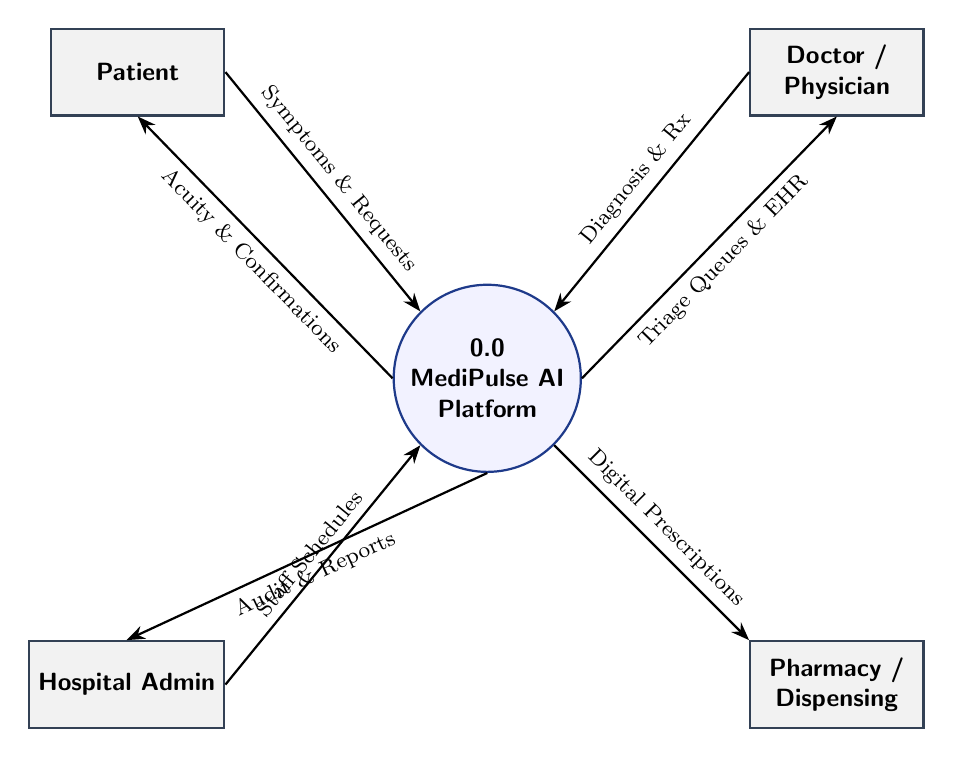
\begin{tikzpicture}[node distance=3.5cm]
    % Central System
    \node[dfdProcess] (system) {\textbf{0.0}\\\textbf{MediPulse AI}\\\textbf{Platform}};
    
    % External Entities
    \node[dfdEntity, above left=of system] (patient) {\textbf{Patient}};
    \node[dfdEntity, above right=of system] (doctor) {\textbf{Doctor /}\\\textbf{Physician}};
    \node[dfdEntity, below left=of system] (admin) {\textbf{Hospital Admin}};
    \node[dfdEntity, below right=of system] (pharmacy) {\textbf{Pharmacy /}\\\textbf{Dispensing}};

    % Data Flows
    \draw[->, thick] (patient.east) -- node[above, sloped, font=\footnotesize] {Symptoms \& Requests} (system.north west);
    \draw[<-, thick] (patient.south) -- node[below, sloped, font=\footnotesize] {Acuity \& Confirmations} (system.west);
    
    \draw[->, thick] (doctor.west) -- node[above, sloped, font=\footnotesize] {Diagnosis \& Rx} (system.north east);
    \draw[<-, thick] (doctor.south) -- node[below, sloped, font=\footnotesize] {Triage Queues \& EHR} (system.east);
    
    \draw[->, thick] (admin.east) -- node[above, sloped, font=\footnotesize] {Staff Schedules} (system.south west);
    \draw[<-, thick] (admin.north) -- node[below, sloped, font=\footnotesize] {Audit \& Reports} (system.south);
    
    \draw[<-, thick] (pharmacy.north west) -- node[above, sloped, font=\footnotesize] {Digital Prescriptions} (system.south east);
\end{tikzpicture}
\caption{DFD Level 0: System Context Diagram}
\label{fig:dfd_level0}
\end{figure}

\subsubsection{DFD Level 1: Subsystem Decomposition}
The Level 1 DFD (Figure~\ref{fig:dfd_level1}) decomposes the system into four major operational processes and three relational data stores.

\begin{figure}[H]
\centering
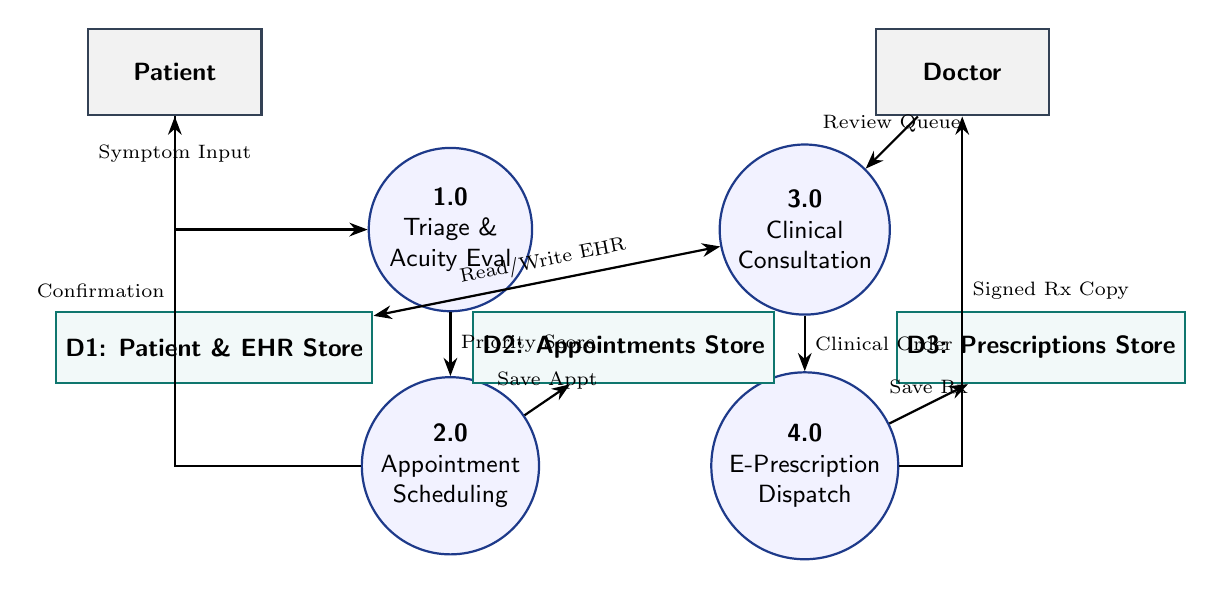
\begin{tikzpicture}[node distance=2.2cm, auto]
    % Entities
    \node[dfdEntity] (pat) at (0, 7) {\textbf{Patient}};
    \node[dfdEntity] (doc) at (10, 7) {\textbf{Doctor}};

    % Processes
    \node[dfdProcess] (p1) at (3.5, 5) {\textbf{1.0}\\Triage \&\\Acuity Eval};
    \node[dfdProcess] (p2) at (3.5, 2) {\textbf{2.0}\\Appointment\\Scheduling};
    \node[dfdProcess] (p3) at (8, 5) {\textbf{3.0}\\Clinical\\Consultation};
    \node[dfdProcess] (p4) at (8, 2) {\textbf{4.0}\\E-Prescription\\Dispatch};

    % Data Stores
    \node[dfdStore] (ds1) at (0.5, 3.5) {\textbf{D1: Patient \& EHR Store}};
    \node[dfdStore] (ds2) at (5.7, 3.5) {\textbf{D2: Appointments Store}};
    \node[dfdStore] (ds3) at (11, 3.5) {\textbf{D3: Prescriptions Store}};

    % Flows
    \draw[->, thick] (pat) |- node[near start, above, font=\scriptsize] {Symptom Input} (p1);
    \draw[->, thick] (p1) -- node[right, font=\scriptsize] {Priority Score} (p2);
    \draw[->, thick] (p2) -- node[above, font=\scriptsize] {Save Appt} (ds2);
    \draw[->, thick] (p2) -| node[near end, left, font=\scriptsize] {Confirmation} (pat);
    
    \draw[->, thick] (doc) -- node[above, font=\scriptsize] {Review Queue} (p3);
    \draw[<->, thick] (p3) -- node[above, sloped, font=\scriptsize] {Read/Write EHR} (ds1);
    \draw[->, thick] (p3) -- node[right, font=\scriptsize] {Clinical Order} (p4);
    \draw[->, thick] (p4) -- node[above, font=\scriptsize] {Save Rx} (ds3);
    \draw[->, thick] (p4) -| node[near end, right, font=\scriptsize] {Signed Rx Copy} (doc);
\end{tikzpicture}
\caption{DFD Level 1: Subsystem Process Decomposition}
\label{fig:dfd_level1}
\end{figure}

\subsection{Use Case Diagram}
Figure~\ref{fig:use_case} details user actors, primary use cases, and behavioral dependencies (\texttt{<<include>>} and \texttt{<<extend>>}).

\begin{figure}[H]
\centering
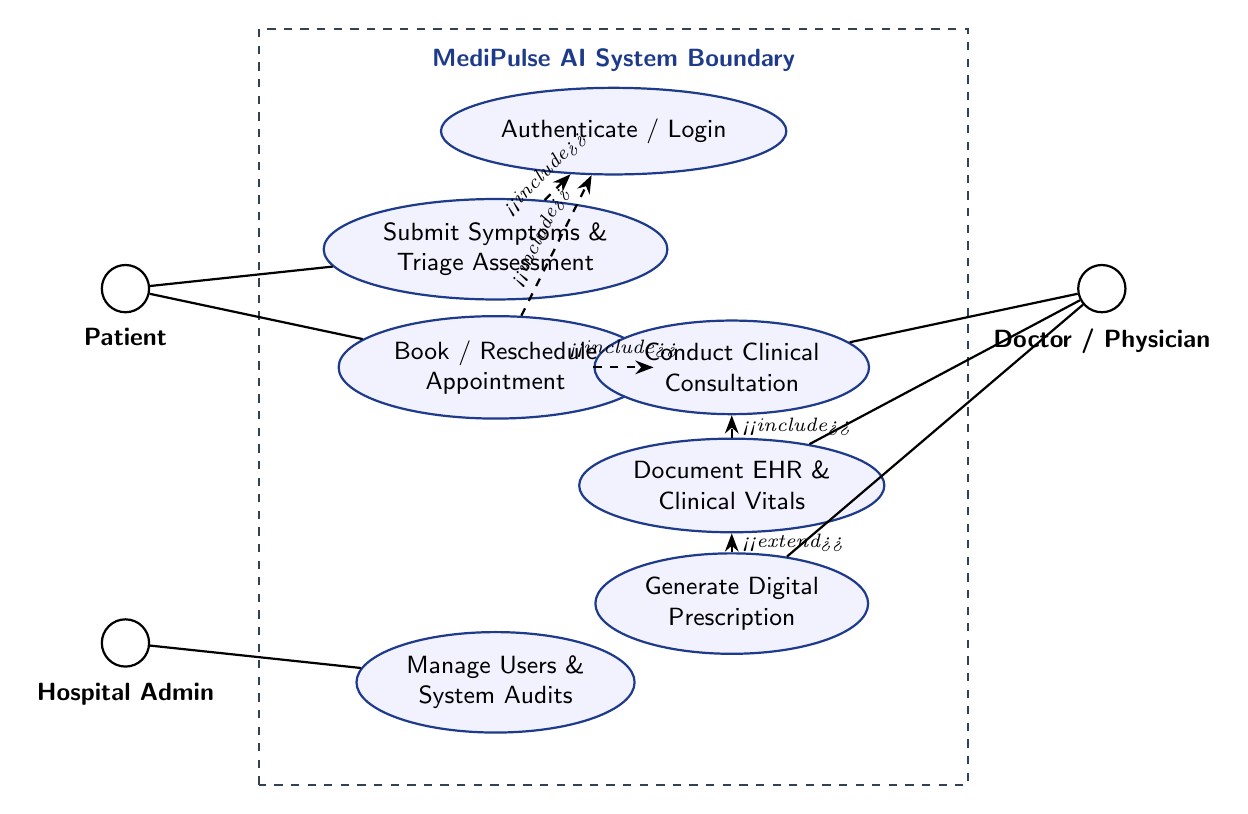
\begin{tikzpicture}
    % System boundary box
    \draw[systembox] (-1.5, -4.8) rectangle (7.5, 4.8);
    \node at (3, 4.4) {\textbf{\color{primaryblue} MediPulse AI System Boundary}};

    % Actors
    \node[actor] (actPatient) at (-3.2, 1.5) {};
    \node[below=2pt of actPatient] {\textbf{Patient}};
    
    \node[actor] (actDoctor) at (9.2, 1.5) {};
    \node[below=2pt of actDoctor] {\textbf{Doctor / Physician}};

    \node[actor] (actAdmin) at (-3.2, -3) {};
    \node[below=2pt of actAdmin] {\textbf{Hospital Admin}};

    % Use Cases
    \node[usecase] (ucAuth) at (3, 3.5) {Authenticate / Login};
    \node[usecase] (ucTriage) at (1.5, 2.0) {Submit Symptoms \&\\Triage Assessment};
    \node[usecase] (ucBook) at (1.5, 0.5) {Book / Reschedule\\Appointment};
    \node[usecase] (ucConsult) at (4.5, 0.5) {Conduct Clinical\\Consultation};
    \node[usecase] (ucEHR) at (4.5, -1.0) {Document EHR \&\\Clinical Vitals};
    \node[usecase] (ucRx) at (4.5, -2.5) {Generate Digital\\Prescription};
    \node[usecase] (ucManage) at (1.5, -3.5) {Manage Users \&\\System Audits};

    % Actor associations
    \draw[thick] (actPatient) -- (ucTriage);
    \draw[thick] (actPatient) -- (ucBook);
    \draw[thick] (actDoctor) -- (ucConsult);
    \draw[thick] (actDoctor) -- (ucEHR);
    \draw[thick] (actDoctor) -- (ucRx);
    \draw[thick] (actAdmin) -- (ucManage);

    % Include / Extend Relationships
    \draw[->, dashed, thick] (ucTriage) -- node[above, sloped, font=\scriptsize] {\textit{<<include>>}} (ucAuth);
    \draw[->, dashed, thick] (ucBook) -- node[above, sloped, font=\scriptsize] {\textit{<<include>>}} (ucAuth);
    \draw[->, dashed, thick] (ucConsult) -- node[above, sloped, font=\scriptsize] {\textit{<<include>>}} (ucBook);
    \draw[->, dashed, thick] (ucEHR) -- node[right, font=\scriptsize] {\textit{<<include>>}} (ucConsult);
    \draw[->, dashed, thick] (ucRx) -- node[right, font=\scriptsize] {\textit{<<extend>>}} (ucEHR);
\end{tikzpicture}
\caption{UML Use Case Diagram with Include and Extend Relationships}
\label{fig:use_case}
\end{figure}

\subsection{Activity Diagram}
Figure~\ref{fig:activity_diagram} models the business logic workflow of patient self-assessment, triage branch decisioning, doctor consultation, and prescription issuance.

\begin{figure}[H]
\centering
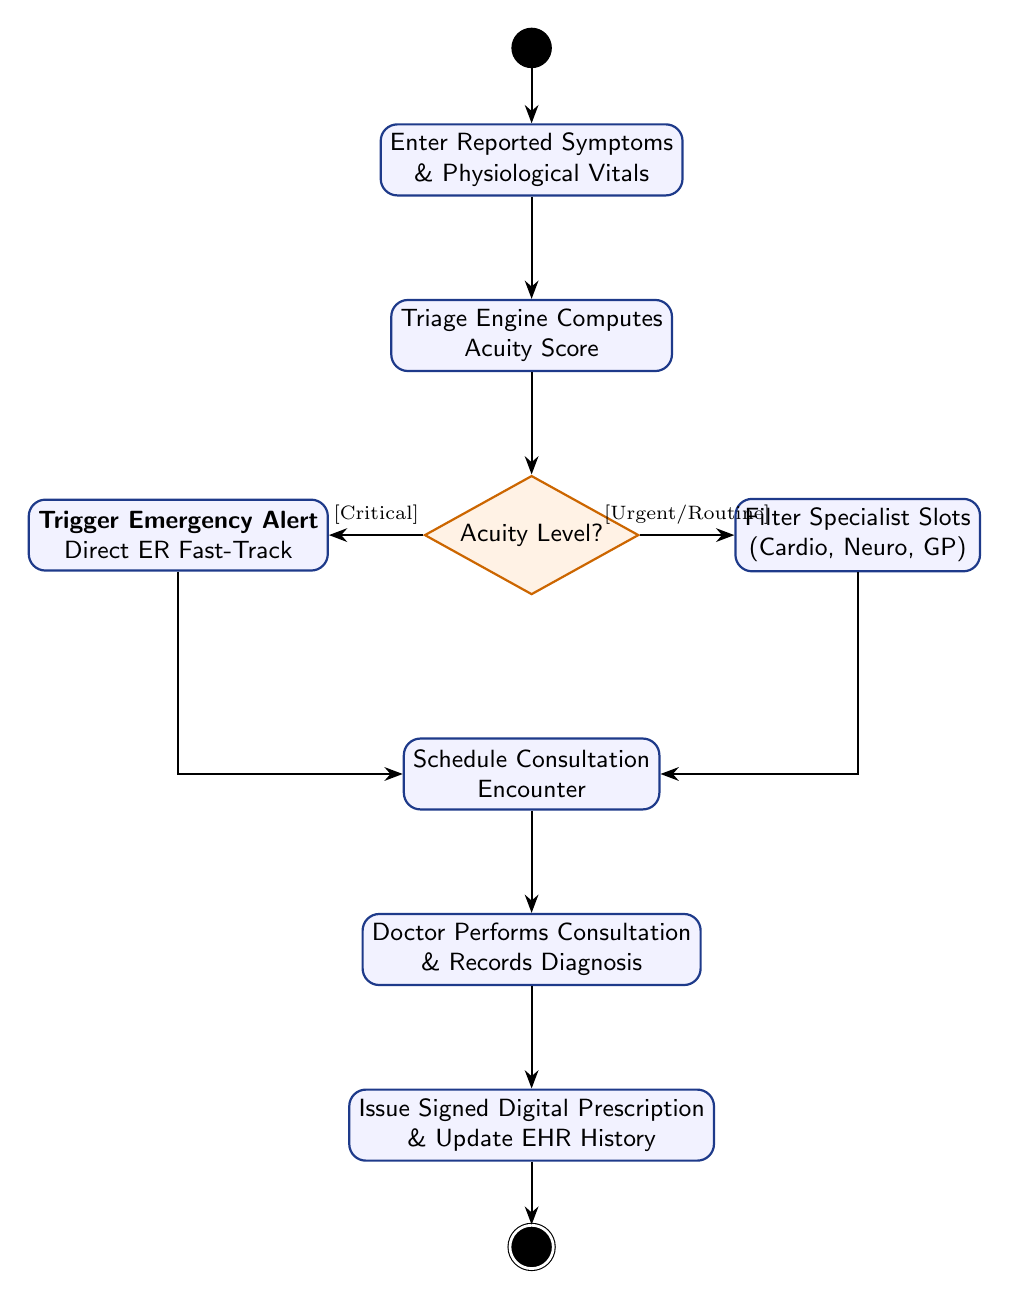
\begin{tikzpicture}[node distance=1.3cm]
    % Nodes
    \node[activityStart] (start) {};
    \node[activityAction, below=0.7cm of start] (input) {Enter Reported Symptoms\\\& Physiological Vitals};
    \node[activityAction, below=of input] (eval) {Triage Engine Computes\\Acuity Score};
    \node[activityDecision, below=of eval] (dec) {Acuity Level?};
    
    \node[activityAction, left=1.2cm of dec] (erAlert) {\textbf{Trigger Emergency Alert}\\Direct ER Fast-Track};
    \node[activityAction, right=1.2cm of dec] (routine) {Filter Specialist Slots\\(Cardio, Neuro, GP)};
    
    \node[activityAction, below=1.8cm of dec] (book) {Schedule Consultation\\Encounter};
    \node[activityAction, below=of book] (consult) {Doctor Performs Consultation\\\& Records Diagnosis};
    \node[activityAction, below=of consult] (issue) {Issue Signed Digital Prescription\\\& Update EHR History};
    \node[activityEnd, below=0.8cm of issue] (stop) {};

    % Connectors
    \draw[->, thick] (start) -- (input);
    \draw[->, thick] (input) -- (eval);
    \draw[->, thick] (eval) -- (dec);
    
    \draw[->, thick] (dec) -- node[above, font=\scriptsize] {[Critical]} (erAlert);
    \draw[->, thick] (dec) -- node[above, font=\scriptsize] {[Urgent/Routine]} (routine);
    
    \draw[->, thick] (erAlert) |- (book);
    \draw[->, thick] (routine) |- (book);
    
    \draw[->, thick] (book) -- (consult);
    \draw[->, thick] (consult) -- (issue);
    \draw[->, thick] (issue) -- (stop);
\end{tikzpicture}
\caption{UML Activity Diagram for Clinical Consultation and Triage Workflow}
\label{fig:activity_diagram}
\end{figure}

\subsection{Entity-Relationship Diagram (ERD)}
Figure~\ref{fig:erd_diagram} exhibits the logical database schema in Crow's Foot notation, exhibiting primary keys (PK), foreign keys (FK), and cardinality.

\begin{figure}[H]
\centering
\begin{tikzpicture}[node distance=3.2cm]
    % Entities
    \node[umlClass] (patient) {
        \textbf{PATIENT}\\
        \midrule
        \underline{patient\_id} (PK) : VARCHAR\\
        name : VARCHAR(100)\\
        dob : DATE\\
        blood\_group : VARCHAR(5)\\
        insurance\_id : VARCHAR(50)
    };

    \node[umlClass, right=2.5cm of patient] (doctor) {
        \textbf{DOCTOR}\\
        \midrule
        \underline{doctor\_id} (PK) : VARCHAR\\
        name : VARCHAR(100)\\
        specialization : VARCHAR(80)\\
        license\_no : VARCHAR(50)\\
        consultation\_fee : DECIMAL(8,2)
    };

    \node[umlClass, below=2.0cm of patient] (appointment) {
        \textbf{APPOINTMENT}\\
        \midrule
        \underline{appointment\_id} (PK) : VARCHAR\\
        \textit{patient\_id} (FK) : VARCHAR\\
        \textit{doctor\_id} (FK) : VARCHAR\\
        date\_time : TIMESTAMP\\
        triage\_priority : VARCHAR(20)\\
        status : VARCHAR(20)
    };

    \node[umlClass, below=2.0cm of doctor] (medical_record) {
        \textbf{MEDICAL\_RECORD}\\
        \midrule
        \underline{record\_id} (PK) : VARCHAR\\
        \textit{patient\_id} (FK) : VARCHAR\\
        \textit{doctor\_id} (FK) : VARCHAR\\
        diagnosis : TEXT\\
        vitals : JSONB\\
        treatment\_plan : TEXT
    };

    \node[umlClass, below=2.0cm of appointment] (prescription) {
        \textbf{PRESCRIPTION}\\
        \midrule
        \underline{prescription\_id} (PK) : VARCHAR\\
        \textit{appointment\_id} (FK) : VARCHAR\\
        \textit{patient\_id} (FK) : VARCHAR\\
        medications : JSONB\\
        instructions : TEXT\\
        is\_dispensed : BOOLEAN
    };

    % Relationships with Crow's Foot annotations
    \draw[thick] (patient) -- node[left, font=\scriptsize] {1} (appointment) node[right, near end, font=\scriptsize] {0..*};
    \draw[thick] (doctor) -- node[left, font=\scriptsize] {1} (appointment) node[right, near end, font=\scriptsize] {0..*};
    
    \draw[thick] (patient) -- node[above, font=\scriptsize] {1} (medical_record) node[above, near end, font=\scriptsize] {0..*};
    \draw[thick] (doctor) -- node[right, font=\scriptsize] {1} (medical_record) node[right, near end, font=\scriptsize] {0..*};
    
    \draw[thick] (appointment) -- node[left, font=\scriptsize] {1} (prescription) node[left, near end, font=\scriptsize] {0..1};
\end{tikzpicture}
\caption{Entity-Relationship Diagram (ERD) with Keys and Cardinality}
\label{fig:erd_diagram}
\end{figure}

\subsection{UML Class Diagram}
Figure~\ref{fig:class_diagram} details the object-oriented structure of the domain model. It highlights generalization (inheritance), associations, typed attributes with visibility indicators (\texttt{+} for public, \texttt{-} for private, \texttt{\#} for protected), and method signatures.

\begin{figure}[H]
\centering
\begin{tikzpicture}[node distance=2.2cm]
    % Base User Class
    \node[umlClass, minimum width=6cm] (user) at (5, 9) {
        \textbf{<<Abstract>> User}\\
        \midrule
        \# user\_id : String\\
        \# name : String\\
        \# email : String\\
        \# phone : String\\
        \# role : String\\
        \midrule
        + get\_dashboard\_summary() : Dict\\
        + to\_dict() : Dict
    };

    % Subclasses: Patient and Doctor
    \node[umlClass, minimum width=4.5cm] (patient) at (1.5, 4.8) {
        \textbf{Patient}\\
        \midrule
        + dob : String\\
        + blood\_group : String\\
        + insurance\_id : String\\
        + records : List<MedicalRecord>\\
        + prescriptions : List<Prescription>\\
        \midrule
        + add\_record(rec: MedicalRecord) : void\\
        + add\_prescription(rx: Prescription) : void\\
        + get\_dashboard\_summary() : Dict
    };

    \node[umlClass, minimum width=4.8cm] (doctor) at (8.5, 4.8) {
        \textbf{Doctor}\\
        \midrule
        + specialization : String\\
        + license\_number : String\\
        + consultation\_fee : Float\\
        + scheduled\_appts : List<Appointment>\\
        \midrule
        + conduct\_consultation(...) : MedicalRecord\\
        + issue\_prescription(...) : Prescription\\
        + get\_dashboard\_summary() : Dict
    };

    % Supporting Classes
    \node[umlClass, minimum width=5.2cm] (appt) at (1.5, 0.2) {
        \textbf{Appointment}\\
        \midrule
        + appointment\_id : String\\
        + patient : Patient\\
        + doctor : Doctor\\
        + date\_time : String\\
        + triage\_priority : String\\
        + status : String\\
        \midrule
        + reschedule(new\_time: String) : void\\
        + complete() : void\\
        + cancel() : void
    };

    \node[umlClass, minimum width=5.2cm] (record) at (8.5, 0.2) {
        \textbf{MedicalRecord}\\
        \midrule
        + record\_id : String\\
        + patient : Patient\\
        + doctor : Doctor\\
        + diagnosis : String\\
        + vitals : Dict<String, String>\\
        + treatment\_plan : String\\
        \midrule
        + to\_dict() : Dict
    };

    \node[umlClass, minimum width=5.2cm] (rx) at (5, -3.8) {
        \textbf{Prescription}\\
        \midrule
        + prescription\_id : String\\
        + appointment\_id : String\\
        + patient : Patient\\
        + doctor : Doctor\\
        + medications : List<Dict>\\
        + instructions : String\\
        + is\_dispensed : Boolean\\
        \midrule
        + dispense() : void\\
        + to\_dict() : Dict
    };

    \node[umlClass, minimum width=4cm] (triage) at (-3.2, 2.5) {
        \textbf{TriageEngine}\\
        \midrule
        - version : String\\
        - rules : Dict\\
        \midrule
        + evaluate(...) : Dict\\
        + get\_specialty(...) : String
    };

    % Inheritance Arrows (Triangle Head)
    \draw[-{Triangle[open]}, thick] (patient.north) -- ++(0, 0.8) -| (user.south west);
    \draw[-{Triangle[open]}, thick] (doctor.north) -- ++(0, 0.8) -| (user.south east);

    % Associations
    \draw[thick] (patient) -- node[left, font=\scriptsize] {1} (appt) node[left, font=\scriptsize, near end] {0..*};
    \draw[thick] (doctor) -- node[right, font=\scriptsize] {1} (appt) node[right, font=\scriptsize, near end] {0..*};
    
    \draw[thick] (patient) -- node[above, font=\scriptsize] {1} (record) node[above, font=\scriptsize, near end] {0..*};
    \draw[thick] (appt) -- node[above, font=\scriptsize] {1} (rx) node[above, font=\scriptsize, near end] {0..1};
    \draw[dashed, ->, thick] (patient) -- (triage);
\end{tikzpicture}
\caption{Comprehensive UML Class Diagram with OOP Design Patterns}
\label{fig:class_diagram}
\end{figure}

\subsection{UML Object Diagram}
Figure~\ref{fig:object_diagram} models an explicit snapshot of instantiated objects during a live clinical session, demonstrating runtime states, assigned attribute values, and bidirectional memory linkages.

\begin{figure}[H]
\centering
\begin{tikzpicture}[node distance=2.2cm]
    % Patient Object Instance
    \node[umlObject, minimum width=5.2cm] (objPatient) at (0, 4) {
        \underline{\textbf{patient1 : Patient}}\\
        \midrule
        user\_id = "PAT-10042"\\
        name = "Khalid Mansoor"\\
        blood\_group = "O+"\\
        insurance\_id = "HLTH-88992"
    };

    % Doctor Object Instance
    \node[umlObject, minimum width=5.2cm] (objDoctor) at (8, 4) {
        \underline{\textbf{doctor1 : Doctor}}\\
        \midrule
        user\_id = "DOC-902"\\
        name = "Dr. Eleanor Vance, MD"\\
        specialization = "Cardiology"\\
        consultation\_fee = \$120.00
    };

    % Appointment Object Instance
    \node[umlObject, minimum width=5.2cm] (objAppt) at (0, -0.5) {
        \underline{\textbf{appt1 : Appointment}}\\
        \midrule
        appointment\_id = "APT-2026-9901"\\
        date\_time = "2026-11-02 10:30 AM"\\
        triage\_priority = "CRITICAL"\\
        status = "COMPLETED"
    };

    % Medical Record Object Instance
    \node[umlObject, minimum width=5.2cm] (objRecord) at (8, -0.5) {
        \underline{\textbf{record1 : MedicalRecord}}\\
        \midrule
        record\_id = "MR-7701"\\
        diagnosis = "Stage 2 Hypertension"\\
        vitals = "BP: 165/100, HR: 88"\\
        treatment\_plan = "Amlodipine + Diet"
    };

    % Prescription Object Instance
    \node[umlObject, minimum width=7cm] (objRx) at (4, -4.5) {
        \underline{\textbf{rx1 : Prescription}}\\
        \midrule
        prescription\_id = "RX-4402"\\
        medications = [\{"drug": "Amlodipine", "dose": "5mg"\}]\\
        instructions = "Take 1 tablet daily with morning meal"\\
        is\_dispensed = false
    };

    % Runtime Linkages
    \draw[thick] (objPatient) -- node[left, font=\scriptsize] {requests} (objAppt);
    \draw[thick] (objDoctor) -- node[right, font=\scriptsize] {supervises} (objAppt);
    \draw[thick] (objDoctor) -- node[right, font=\scriptsize] {creates} (objRecord);
    \draw[thick] (objPatient) -- node[above, font=\scriptsize] {owns} (objRecord);
    \draw[thick] (objAppt) -- node[left, font=\scriptsize] {generates} (objRx);
    \draw[thick] (objDoctor) -- node[right, font=\scriptsize] {signs} (objRx);
\end{tikzpicture}
\caption{UML Object Diagram Capturing Runtime Memory State and Linkages}
\label{fig:object_diagram}
\end{figure}

% ==============================================================================
% CHAPTER 5: PROTOTYPE IMPLEMENTATION & INTERFACE
% ==============================================================================
\section{Prototype Implementation \& Interface Design}

\subsection{Mapping Class Models to User Interface Elements}
As mandated by the capstone requirements, an interactive prototype was developed directly operationalizing at least five interconnected classes from the UML Class Diagram:
\begin{enumerate}
    \item \textbf{Class 1: \texttt{Patient}} -- Manages personal demographic records, medical encounter history, and active prescriptions.
    \item \textbf{Class 2: \texttt{Doctor}} -- Exposes physician consultation fees, clinical specialties, and authorization to conduct consultations.
    \item \textbf{Class 3: \texttt{Appointment}} -- Encapsulates triage priorities, clinical slots, and lifecycle statuses (\textit{Scheduled}, \textit{Completed}).
    \item \textbf{Class 4: \texttt{MedicalRecord}} -- Stores formal diagnostic evaluations, physiological vital sign telemetry, and treatment plans.
    \item \textbf{Class 5: \texttt{Prescription}} -- Represents clinical pharmacological orders, instructions, and fulfillment states.
    \item \textbf{Class 6: \texttt{TriageEngine}} -- Automates clinical urgency heuristics and specialist matching based on symptoms.
\end{enumerate}

\subsection{Interface Architecture and User Workflow}
The prototyping deliverable consists of two complementary interfaces located in the \texttt{prototype/} repository directory:
\begin{itemize}
    \item \textbf{Interactive Web Dashboard (\texttt{index.html}, \texttt{app.js}, \texttt{styles.css}):} A responsive, dual-portal web interface providing an integrated Patient Triage portal, Physician Encounter desk, and a Live Runtime Object Inspector.
    \item \textbf{Console Verification Suite (\texttt{main.py}, \texttt{models.py}):} An automated terminal-driven object-oriented workflow demonstrating end-to-end execution of all six domain classes in Python 3.
\end{itemize}

\subsection{Core OOP Domain Logic Excerpt}
Listing~\ref{lst:python_domain} presents the foundational class definitions proving encapsulation, inheritance, and polymorphic abstractions.

\begin{lstlisting}[language=Python, caption={Core OOP Class Definitions in Python (Excerpt from models.py)}, label={lst:python_domain}]
from abc import ABC, abstractmethod
from datetime import datetime
from typing import List, Dict, Optional

class User(ABC):
    """Abstract Base Class demonstrating OOP Abstraction."""
    def __init__(self, user_id: str, name: str, email: str, phone: str, role: str):
        self._user_id = user_id
        self._name = name
        self._email = email
        self._phone = phone
        self._role = role

    @abstractmethod
    def get_dashboard_summary(self) -> Dict[str, str]:
        pass

class Patient(User):
    """Class 1: Patient Entity inheriting from User."""
    def __init__(self, user_id: str, name: str, email: str, phone: str, 
                 dob: str, blood_group: str, insurance_id: str):
        super().__init__(user_id, name, email, phone, role="PATIENT")
        self.dob = dob
        self.blood_group = blood_group
        self.insurance_id = insurance_id
        self.medical_records: List['MedicalRecord'] = []
        self.prescriptions: List['Prescription'] = []

    def get_dashboard_summary(self) -> Dict[str, str]:
        return {
            "User Type": "Patient",
            "Name": self._name,
            "Records Count": str(len(self.medical_records))
        }

class Doctor(User):
    """Class 2: Doctor Entity inheriting from User."""
    def __init__(self, user_id: str, name: str, email: str, phone: str,
                 specialization: str, license_number: str, consultation_fee: float):
        super().__init__(user_id, name, email, phone, role="DOCTOR")
        self.specialization = specialization
        self.license_number = license_number
        self.consultation_fee = consultation_fee

    def conduct_consultation(self, appointment: 'Appointment', diagnosis: str, 
                             vitals: Dict[str, str], plan: str) -> 'MedicalRecord':
        record = MedicalRecord(f"MR-{uuid.uuid4().hex[:6]}", appointment.patient, 
                               self, diagnosis, vitals, plan)
        appointment.patient.medical_records.append(record)
        appointment.complete()
        return record
\end{lstlisting}

\subsection{Interactive Interface Prototyping Layout}
Figure~\ref{fig:ui_wireframe} details the conceptual layout of the interactive web prototype interface.

\begin{figure}[H]
\centering
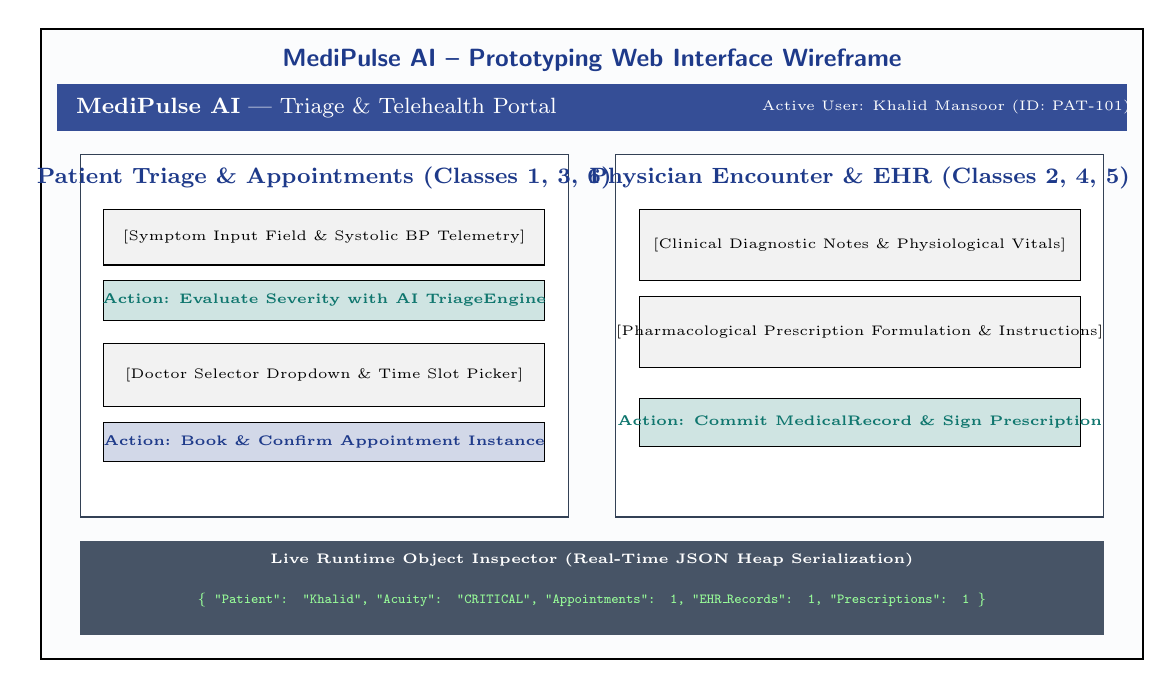
\begin{tikzpicture}
    % Outer Frame
    \draw[thick, fill=lightgray!30] (0, 0) rectangle (14, 8);
    \node at (7, 7.6) {\textbf{\color{primaryblue} MediPulse AI -- Prototyping Web Interface Wireframe}};
    
    % Header
    \draw[fill=primaryblue!90, draw=none] (0.2, 6.7) rectangle (13.8, 7.3);
    \node[white, font=\footnotesize] at (3.5, 7.0) {\textbf{MediPulse AI} | Triage \& Telehealth Portal};
    \node[white, font=\tiny] at (11.5, 7.0) {Active User: Khalid Mansoor (ID: PAT-101)};

    % Left Panel: Patient Triage & Booking
    \draw[fill=white, draw=darkgray] (0.5, 1.8) rectangle (6.7, 6.4);
    \node[primaryblue, font=\footnotesize\bfseries] at (3.6, 6.1) {Patient Triage \& Appointments (Classes 1, 3, 6)};
    
    \draw[fill=gray!10] (0.8, 5.0) rectangle (6.4, 5.7);
    \node[font=\tiny] at (3.6, 5.35) {[Symptom Input Field \& Systolic BP Telemetry]};
    
    \draw[fill=secondaryteal!20] (0.8, 4.3) rectangle (6.4, 4.8);
    \node[font=\tiny\bfseries, color=secondaryteal] at (3.6, 4.55) {Action: Evaluate Severity with AI TriageEngine};

    \draw[fill=gray!10] (0.8, 3.2) rectangle (6.4, 4.0);
    \node[font=\tiny] at (3.6, 3.6) {[Doctor Selector Dropdown \& Time Slot Picker]};

    \draw[fill=primaryblue!20] (0.8, 2.5) rectangle (6.4, 3.0);
    \node[font=\tiny\bfseries, color=primaryblue] at (3.6, 2.75) {Action: Book \& Confirm Appointment Instance};

    % Right Panel: Doctor Encounter & EHR
    \draw[fill=white, draw=darkgray] (7.3, 1.8) rectangle (13.5, 6.4);
    \node[primaryblue, font=\footnotesize\bfseries] at (10.4, 6.1) {Physician Encounter \& EHR (Classes 2, 4, 5)};
    
    \draw[fill=gray!10] (7.6, 4.8) rectangle (13.2, 5.7);
    \node[font=\tiny] at (10.4, 5.25) {[Clinical Diagnostic Notes \& Physiological Vitals]};
    
    \draw[fill=gray!10] (7.6, 3.7) rectangle (13.2, 4.6);
    \node[font=\tiny] at (10.4, 4.15) {[Pharmacological Prescription Formulation \& Instructions]};

    \draw[fill=secondaryteal!20] (7.6, 2.7) rectangle (13.2, 3.3);
    \node[font=\tiny\bfseries, color=secondaryteal] at (10.4, 3.0) {Action: Commit MedicalRecord \& Sign Prescription};

    % Bottom Panel: Live Runtime Object Inspector
    \draw[fill=darkgray!90, draw=none] (0.5, 0.3) rectangle (13.5, 1.5);
    \node[white, font=\tiny\bfseries] at (7, 1.25) {Live Runtime Object Inspector (Real-Time JSON Heap Serialization)};
    \node[green!40, font=\ttfamily\tiny] at (7, 0.75) {\{ "Patient": "Khalid", "Acuity": "CRITICAL", "Appointments": 1, "EHR\_Records": 1, "Prescriptions": 1 \}};
\end{tikzpicture}
\caption{User Interface Prototype Wireframe and Class Functional Mapping}
\label{fig:ui_wireframe}
\end{figure}

% ==============================================================================
% CHAPTER 6: QUALITY ASSURANCE, RISK MANAGEMENT & SECURITY
% ==============================================================================
\section{Quality Assurance, Risk Management \& Security}

\subsection{Testing and Quality Assurance Strategy}
To guarantee system stability, a multi-tiered testing regimen is enforced throughout each sprint iteration:
\begin{itemize}
    \item \textbf{Unit Testing (PyTest \& Jest):} Validates individual class methods, boundary checking on clinical vitals, and correct state transitions.
    \item \textbf{Integration Testing:} Ensures proper data flow between the \texttt{TriageEngine}, \texttt{Appointment} booking queue, and \texttt{MedicalRecord} database.
    \item \textbf{Security and HIPAA Compliance Auditing:} Verifies cryptographic hashing of authentication tokens and end-to-end payload sanitization.
\end{itemize}

\subsection{Risk Assessment and Mitigation Matrix}
Table~\ref{tab:risk_matrix} categorizes identified project risks, assessed severity, and proactive mitigation protocols.

\begin{table}[H]
\centering
\caption{Comprehensive Project Risk Assessment and Mitigation Matrix}
\label{tab:risk_matrix}
\small
\begin{tabularx}{\textwidth}{lp{3.5cm}ccX}
\toprule
\textbf{Risk ID} & \textbf{Risk Description} & \textbf{Probability} & \textbf{Impact} & \textbf{Mitigation Strategy} \\
\midrule
\textbf{R-01} & Clinical triage false-negative score on acute conditions. & Low & Critical & Conservative rule-based physiological overrides (e.g., BP $\ge$ 180 forces CRITICAL rating). \\
\textbf{R-02} & Unsynchronized scheduling conflicts during peak bookings. & Medium & Moderate & Database row-level transactional locks (\texttt{SELECT ... FOR UPDATE}) on appointment slots. \\
\textbf{R-03} & Sensitive Patient Health Information (PHI) exposure. & Low & High & AES-256 database column encryption, TLS 1.3 transport security, strict RBAC authorization. \\
\textbf{R-04} & Scope creep affecting delivery of secondary features. & Medium & Medium & Strict Agile backlog prioritization; delimiting Phase I to verified core classes and UI prototype. \\
\bottomrule
\end{tabularx}
\end{table}

% ==============================================================================
% CHAPTER 7: CONCLUSION & FUTURE WORK
% ==============================================================================
\section{Conclusion \& Future Roadmap}

\subsection{Part I Conclusion}
This Senior Capstone Project Proposal (Part I) establishes a comprehensive, academically rigorous, and industry-aligned foundation for \textbf{MediPulse AI}. By synthesizing Agile Scrum project management, formal Unified Modeling Language artifacts (DFD 0/1, Use Case, Activity, ERD, Class, and Object diagrams), and a fully operational 6-class object-oriented prototype, all criteria for Part I are thoroughly satisfied.

\subsection{Roadmap for Part II (Implementation \& Deployment)}
Following approval of this proposal, Phase II will execute the subsequent milestones:
\begin{enumerate}
    \item \textbf{Phase II Sprint 4:} Containerization via Docker and Kubernetes microservices deployment.
    \item \textbf{Phase II Sprint 5:} Real-time WebSocket bidirectional tele-consultation audio/video channels.
    \item \textbf{Phase II Sprint 6:} Clinical field pilot testing, institutional review, and final capstone thesis defense.
\end{enumerate}

% ==============================================================================
% REFERENCES
% ==============================================================================
\newpage
\bibliographystyle{IEEEtran}
\bibliography{references}

% ==============================================================================
% APPENDIX: REPOSITORY SUBMISSION & CODE LISTINGS
% ==============================================================================
\newpage
\appendix
\section{GitHub Repository Organization \& Reproduction Guide}
As required by the submission guidelines (\textit{``Submit: Proposal containing all the requirements above (GitHub Link)''}), all source code, models, and interactive interfaces are structured in the submission repository as follows:

\begin{verbatim}
medipulse-ai-capstone/
|-- proposal.tex              # Master LaTeX Document (This Paper)
|-- references.bib            # BibTeX References Database
|-- proposal.html             # Standalone Compiled Publication Report
|-- README.md                 # Complete GitHub Submission Guide & Video Walkthrough
`-- prototype/
    |-- models.py             # Python OOP Classes (User, Patient, Doctor, Appt, etc.)
    |-- main.py               # Interactive Console Demonstration
    |-- index.html            # Web Interface Dashboard
    |-- styles.css            # Responsive Healthcare UI Styling
    `-- app.js                # Frontend Controller Instantiating Domain Classes
\end{verbatim}

\subsection{Local Reproduction Instructions}
\begin{enumerate}
    \item \textbf{Clone the Repository:}
    \begin{verbatim}
    git clone https://github.com/khalid-capstone/medipulse-ai.git
    cd medipulse-ai
    \end{verbatim}
    
    \item \textbf{Run the Python OOP Prototype:}
    \begin{verbatim}
    python prototype/main.py
    \end{verbatim}

    \item \textbf{Launch the Interactive Web Interface:}
    Double-click \texttt{prototype/index.html} or open it in any modern browser (Google Chrome, Firefox, Safari, Microsoft Edge). No external web server is required.

    \item \textbf{Compile LaTeX Proposal to PDF:}
    \begin{verbatim}
    pdflatex proposal.tex
    bibtex proposal
    pdflatex proposal.tex
    pdflatex proposal.tex
    \end{verbatim}
    Alternatively, import this repository directly into Overleaf for one-click compilation.
\end{enumerate}

\end{document}